\documentclass{article}

\usepackage[utf8]{inputenc}
\usepackage{graphicx}		% Graphics.
\usepackage{color}
\usepackage[english]{babel}
\usepackage{float}
\usepackage{subcaption}
\usepackage{xfrac}
\usepackage{matlab-prettifier}
\usepackage{amsmath}    
\usepackage{amssymb}
\usepackage{siunitx}
\usepackage{chemformula}
\usepackage{physics}
\usepackage{pdfpages}
\usepackage{wrapfig}
\usepackage[justification=centering]{caption}

% Create a separate table for the appendix.
\usepackage[toc,page]{appendix}

% Table of Content has fast links to sections.
\usepackage{hyperref}

% Remove dots in table of contents.
\usepackage[titles]{tocloft}
\renewcommand{\cftdot}{}

% Page style.
\usepackage[top=2cm, bottom=2cm, left = 2cm, right = 2cm]{geometry}
\setlength{\parindent}{0pt}	% Disable indents.

% BIBTEX.
\usepackage[style=ieee]{biblatex}
\usepackage{csquotes}
\addbibresource{references.bib}

\begin{document}

%----------------------------------------------------------------------------------------
%	Title page.
%----------------------------------------------------------------------------------------
%----------------------------------------------------------------------------------------
%	TITLE PAGE.
%----------------------------------------------------------------------------------------

\begin{titlepage} % Suppresses displaying the page number on the title page and the subsequent page counts as page 1.
	\center % Centre everything on the page.
	\newcommand{\HRule}{\rule{\linewidth}{0.5mm}} % Defines a new command for horizontal lines, change thickness here.
	
	
	%------------------------------------------------
	%	Logo.
	%------------------------------------------------
	
\includegraphics[width=0.4\textwidth, trim=0 0 0 -2cm]{figures/LTU_logo.jpg}\\[1cm]
		
	
	%------------------------------------------------
	%	Headings.
	%------------------------------------------------
	\textsc{\Huge Lule\aa \ University of Technology}\\[1.5cm]
	
	\textsc{\LARGE Polar Atmospheric Physics}\\[0.3cm]
	
	\textsc{\large F7014R}\\[0.5cm]
	
	
	%------------------------------------------------
	%	Title.
	%------------------------------------------------
	\HRule\\[0.4cm]
	
	{\Huge\bfseries EISCAT Space Weather}\\[0.4cm]
	
	\HRule\\[1.5cm]
	
	
	%------------------------------------------------
	%	Author & supervisor.
	%------------------------------------------------
	\begin{minipage}{0.4\textwidth}
		\begin{flushleft}
			\large
			\textit{Authors}\\
			D. Talavera\\
			E.F.M. Weterings\\
		\end{flushleft}
	\end{minipage}
	~
	\begin{minipage}{0.4\textwidth}
		\begin{flushright}
			\large
			\textit{Supervisors}\\
			A. Tjulin\\
			C.F. Enell\\
			V. Barabash
		\end{flushright}
	\end{minipage}
	
	
	%------------------------------------------------
	%	Date.
	%------------------------------------------------
	\vfill\vfill\vfill % Position the date 3/4 down the remaining page.
	
	{\large\today} % Date, change the \today to a set date if you want to be precise.
	
	
\end{titlepage}


%----------------------------------------------------------------------------------------
%	TABLE OF CONTENT.
%----------------------------------------------------------------------------------------
\newpage				% Start at new page.
\pagenumbering{arabic}	% Page numbering reset & style.
\renewcommand{\contentsname}{Table of Contents}
\tableofcontents		% Add table of content.


%----------------------------------------------------------------------------------------
%	INTRODUCTION (1).
%----------------------------------------------------------------------------------------
\newpage
%----------------------------------------------------------------------------------------
%	INTRODUCTION.
%----------------------------------------------------------------------------------------
%example MISC \cite{exampleMISC}.\\
%example Book \cite{exampleBOOK}.\\
%example article \cite[p.~5]{exampleARTICLE}

\section{Introduction}
The purpose of this report is to relate space weather events with analyzed data from EISCAT.
The end result of this practical is to become acquainted with data from EISCAT and the programs used to analyze it.
This report will be analyzing data from the EISCAT radar through the use of GUISDAP. 
The pre-analyzed data comes from EISCAT through Madrigal database.
With GUISDAP and Madrigal, the plots will be interpreted to find relationships with space weather. \\

The effect from the sun and the other extraplanetary sources on the Earth is called space weather. 
The influence of space weather on Earth include the aurora, disturbances in magnetosphere and ionosphere, and geomagnetic induced currents \cite{I_NOAA_2}. 
The causes of the space weather originates from the sun which includes coronal mass ejections, solar flares, and coronal holes.
There are several effects originating from space weather: damaging spacecraft electronics, increased drag affecting orbit of satellites, increasing radiation dosage in astronauts and airplane passengers, causing radio blackouts on Earth, and causing electrical power grid power outages.
Space weather can be observed by ground-based systems or by satellites. Ground-based systems involve telescopes observing the photosphere, neutron detectors, and measuring the ionosphere.
Many current satellites carry sun monitoring sensors as secondary payloads.
There are mathematical models that can simulate the space weather environment.\\


The space weather event studied mostly in this report occurred between October 19$^{th}$ and November 7$^{th}$ and is referred to as the Halloween solar storms. 
It occurred during the later part of solar cycle 23. It was not expected during the quieter part of the solar cycle.
It had a large affect on Earth, with aurora seen in Florida, satellites and communications being affected, and a power outage is Sweden lasting for a hour \cite{I_NASA_1}. 
It was composed of 17 flares ranging in strength, with the largest being estimated at X28 power causing a R5 radio blackout and numerous anomalies in satellites \cite{I_NOAA}.



%----------------------------------------------------------------------------------------
%	GUISDAP (3).
%----------------------------------------------------------------------------------------
\newpage
%----------------------------------------------------------------------------------------
%	GUISDAP.
%----------------------------------------------------------------------------------------

\section{GUISDAP software}
In this section the raw EISCAT data is processed using the MATLAB software with the package GUISDAP. This is done for the 27th of October 2016 from 18:00 to 19:00. This solar weather event consisted of a series of solar flares and coronal mass ejections. The series of storms were the largest ever recorded by the GOES satellite (Geostationary Operational Environmental Satellite). Satellite-based systems and communications were affected, aircraft were advised to avoid high altitudes near the polar regions, and a one-hour-long power outage occurred in Sweden as a result of the solar activity. Auroras were observed at latitudes as far south as Texas and the Mediterranean countries of Europe.


%----------------------------------------------------------------------------------------
%	SPACEWEATHER EVENT (3).
%----------------------------------------------------------------------------------------
\newpage
%----------------------------------------------------------------------------------------
%	SPACEWEATHER EVENT.
%----------------------------------------------------------------------------------------
\section{Space weather event}
\begin{wrapfigure}[19]{r}{6.5cm}
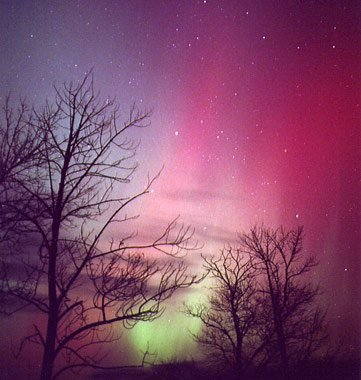
\includegraphics[width=6.5cm]{figures/SW_aurora_29oct_3.jpg}

\caption{Geomagnetic storm/ Aurora on the 29th of October \cite{spaceweather}.}
\label{fig:Aurora3}
\end{wrapfigure} 
In the rest of this document preprocessed data is used from the Halloween 2003 space weather event. This event took place from the 28th up to the 29th of October, with the main two peaks at 11:10 (28-10-2003) and 20:50 (29-10-2003) \cite{goes_x-ray_archive}. This solar weather event consisted of a series of solar flares and coronal mass ejections. The solar flare with the most energy was measured at 10:16:53 UCT. With an energy of $6.9\cdot10^{25}$\,Joule and a mass of $1.6 \cdot 10^{10}$\,gram \cite{CME_list}, one of the strongest ever measured by GOES.\\

Satellite-based systems and communications were affected, as well as the instruments onboard \cite{swpc-noaa}. Aircraft were advised to avoid high altitudes near the polar regions, and a one-hour-long power outage occurred in Sweden as a result of the solar activity. Auroras (figure \ref{fig:Aurora3}) were observed at latitudes as far south as Texas and the Mediterranean countries of Europe \cite{wiki_halloween_solar_stroms}.

\subsection{Solar flares}
\begin{wrapfigure}{r}{0.5\textwidth}
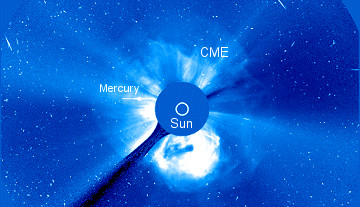
\includegraphics[width=.5\textwidth]{figures/SW_CME.jpg}

\caption{Solar image of a CME using a cronagraph\cite{spaceweather}.}
\label{fig:SW:CME}
\end{wrapfigure} 

On the 28th 12:18 UCT one of the most powerful solar flares in years erupted, this eruption, that caused a intense geomagnetic storm, is shown in figure \ref{fig:SW:CME}.The solar flares erupted out of 486 giant sunspots. It was measured X17  on the Richter scale of solar flares. This means that the peak had an energy above $7 \cdot 10^{-4}$\,W/m$^2$. It was also classified as a S3 storm, which means it has a flux of more than $10^3$ with $\geq$10\,MeV particles.  \cite{spaceweather}.\\


%----------------------------------------------------------------------------------------
%	GOES.
%----------------------------------------------------------------------------------------
\subsection{GOES}
In figure \ref{fig:goes_sem_data_oct} the space weather data from GOES10 (10th Geostationary Operational Environmental Satellite) over the month October is shown. In figure \ref{fig:goes_sem_data_nov} the data from the same satellite is shown over the month of November \cite{ngdc-noaa}. \\

WHAT IS SHOWN HERE!\\

DISCUSSION / INTERPRETATION

\begin{figure}[H]
\centering
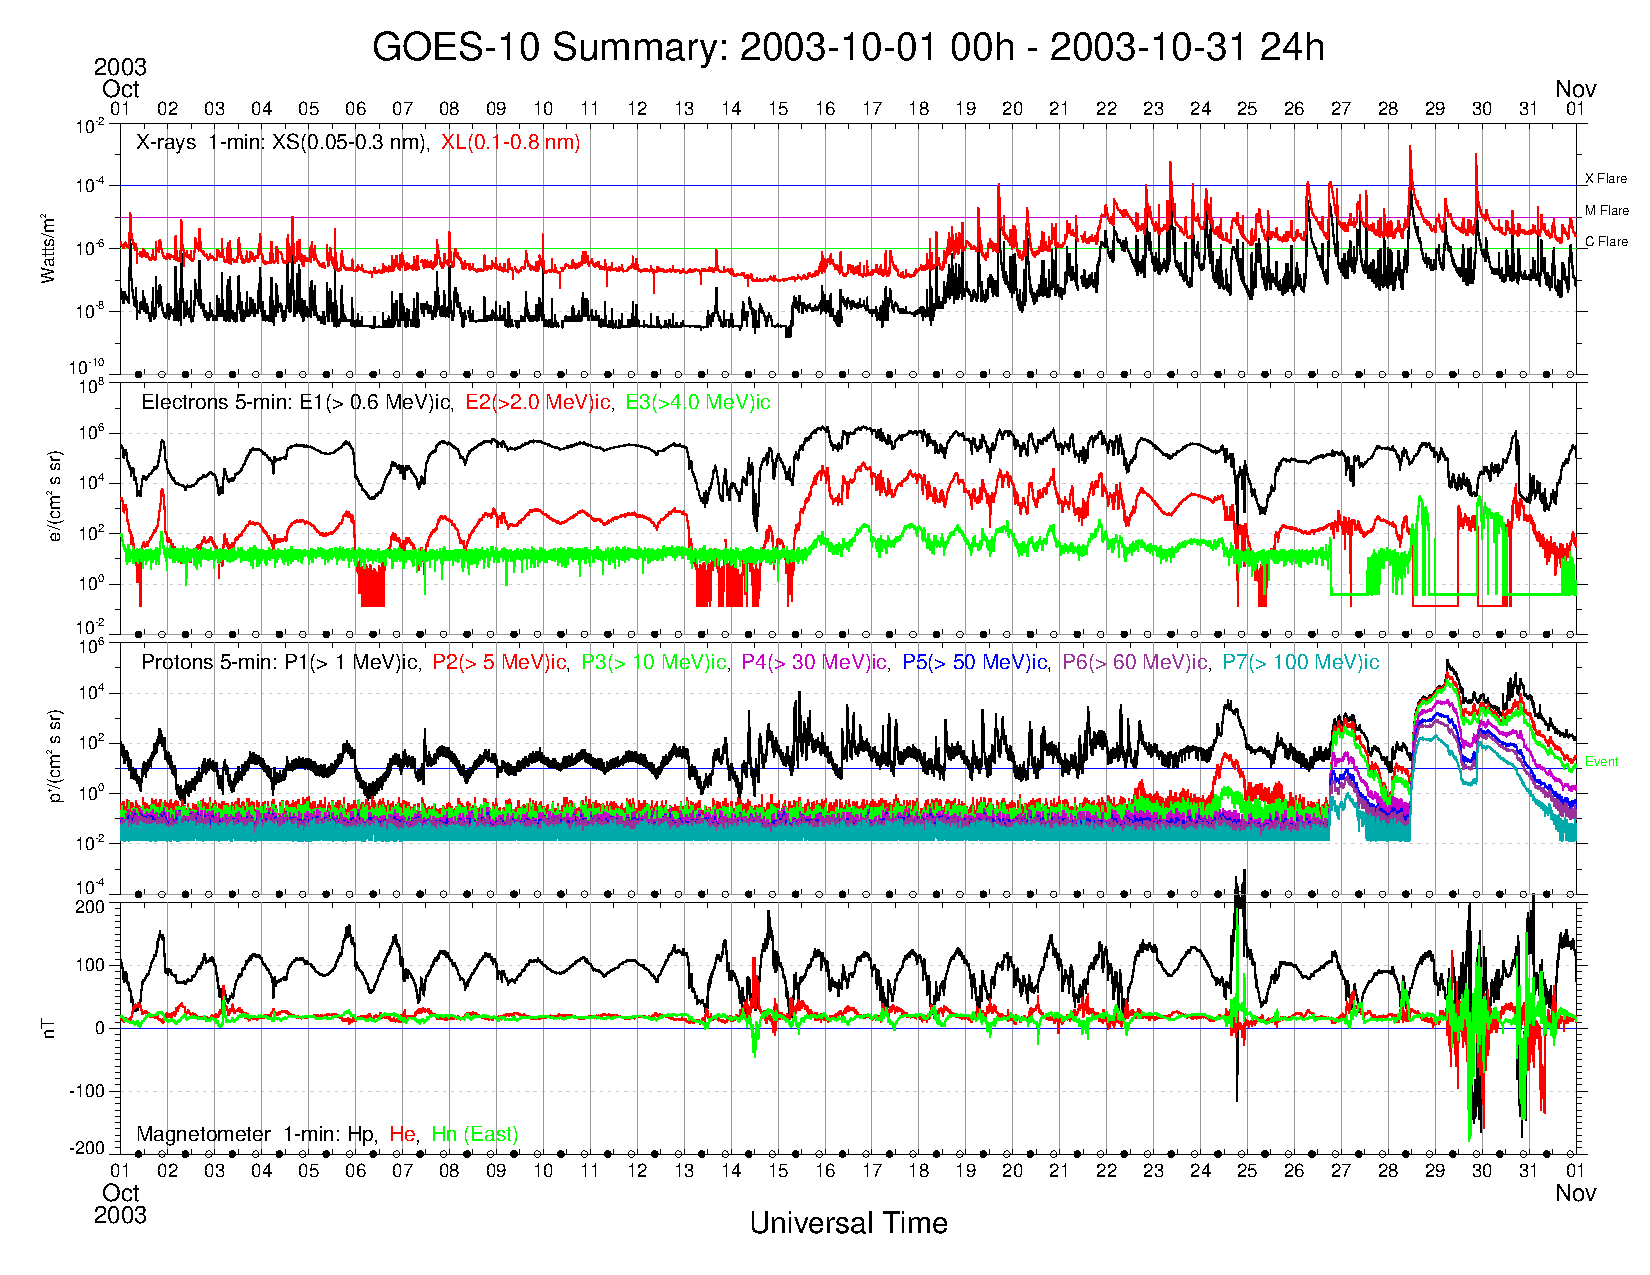
\includegraphics[page=1, width=.79\textwidth]{figures/goes10_oct.pdf}

\caption{\cite{ngdc-noaa}.}
\label{fig:goes_sem_data_oct}
\end{figure}

\begin{figure}[H]
\centering
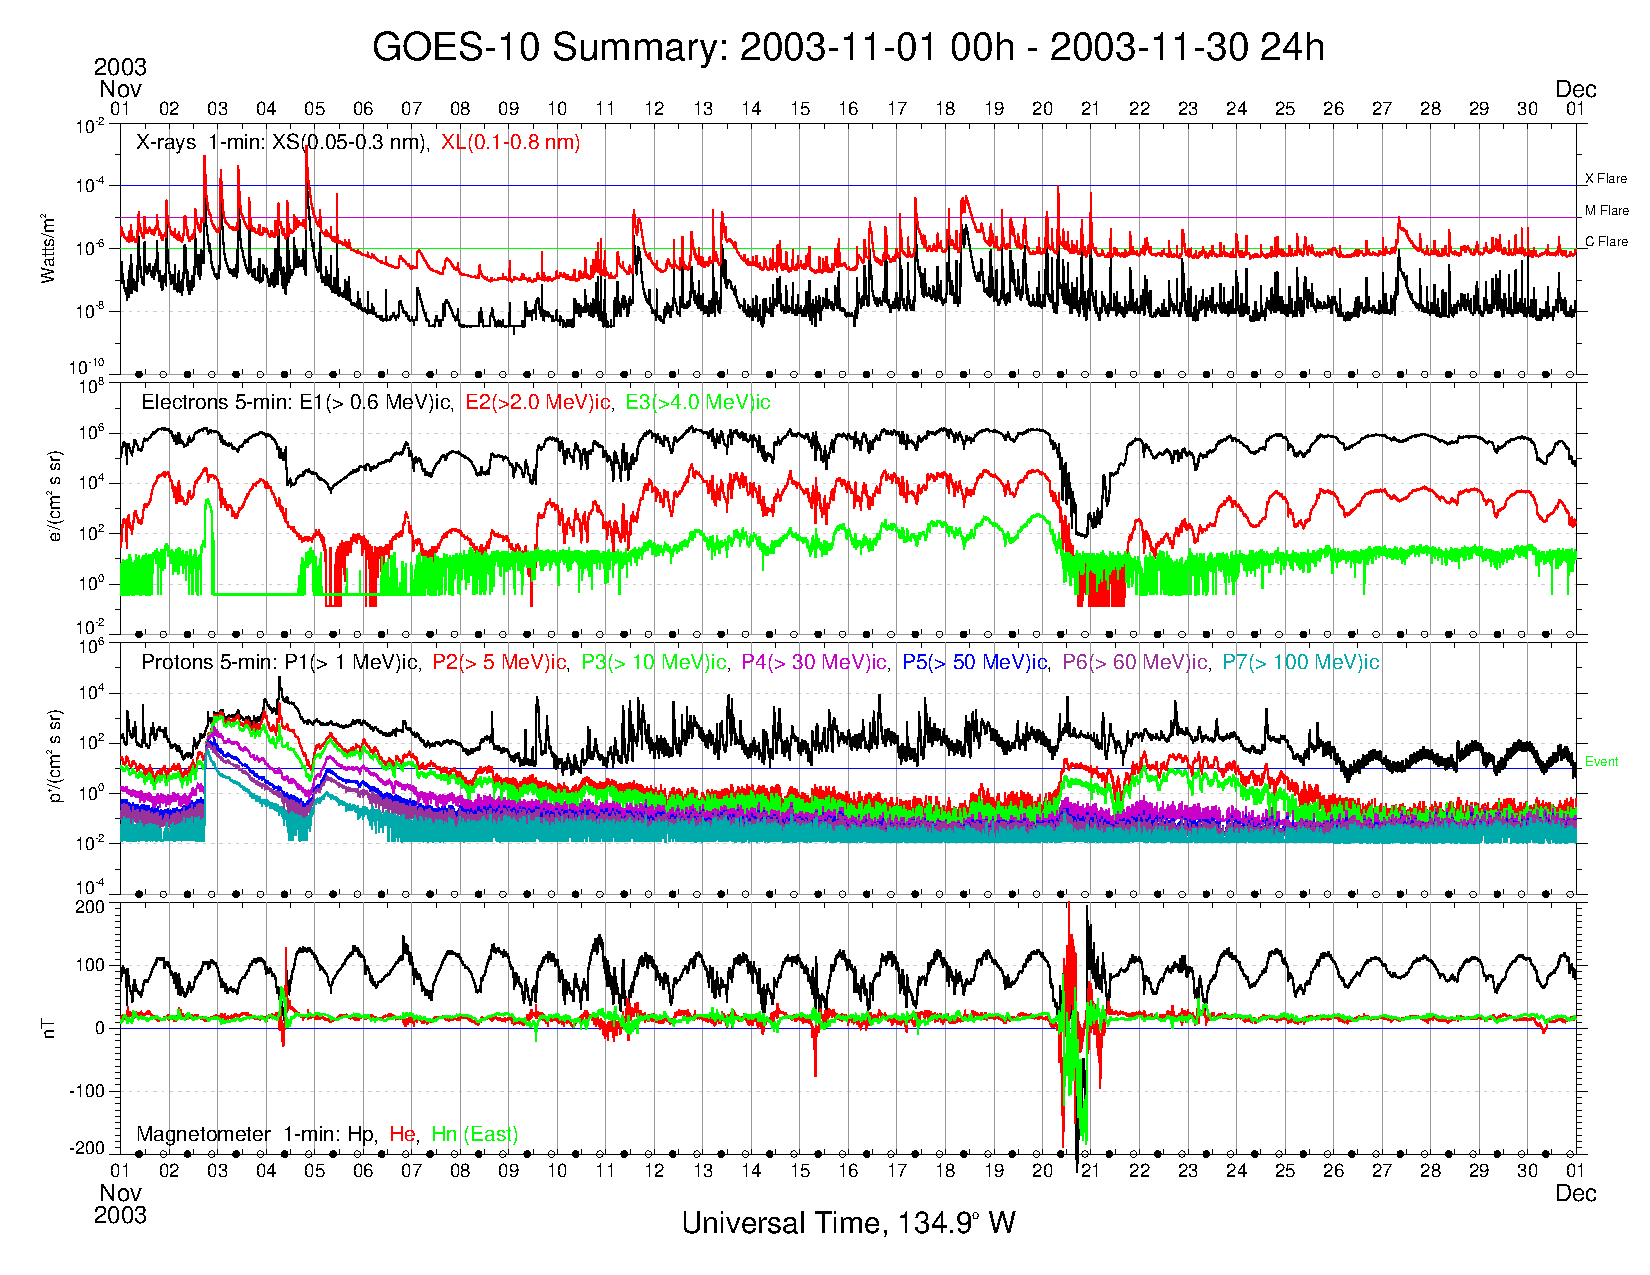
\includegraphics[page=1, width=.79\textwidth]{figures/goes10_nov.pdf}

\caption{\cite{ngdc-noaa}.}
\label{fig:goes_sem_data_nov}
\end{figure}


%----------------------------------------------------------------------------------------
%	IMAGE.
%----------------------------------------------------------------------------------------
\subsection{IMAGE}

text/ explanation

\begin{figure}[H]
        \begin{subfigure}[b]{0.33\textwidth}
                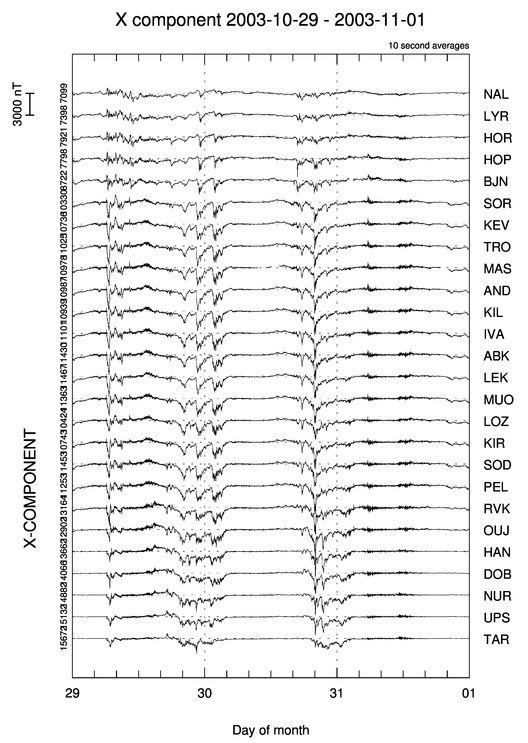
\includegraphics[width=\linewidth]{figures/IMAGE_X_gram.jpg}
                \caption{\cite{image}.}
				\label{fig:image_x_gram}
        \end{subfigure}%
        \begin{subfigure}[b]{0.34\textwidth}
                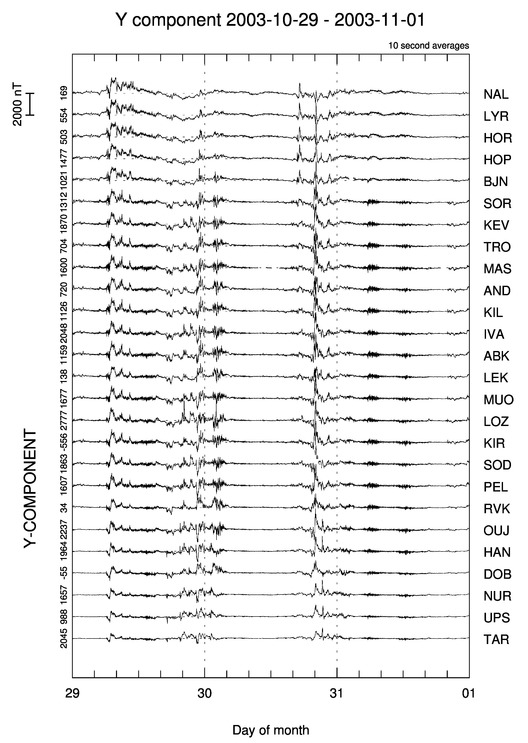
\includegraphics[width=\linewidth]{figures/IMAGE_Y_gram.jpg}
                \caption{\cite{image}.}
				\label{fig:image_y_gram}
        \end{subfigure}%
        \begin{subfigure}[b]{0.33\textwidth}
                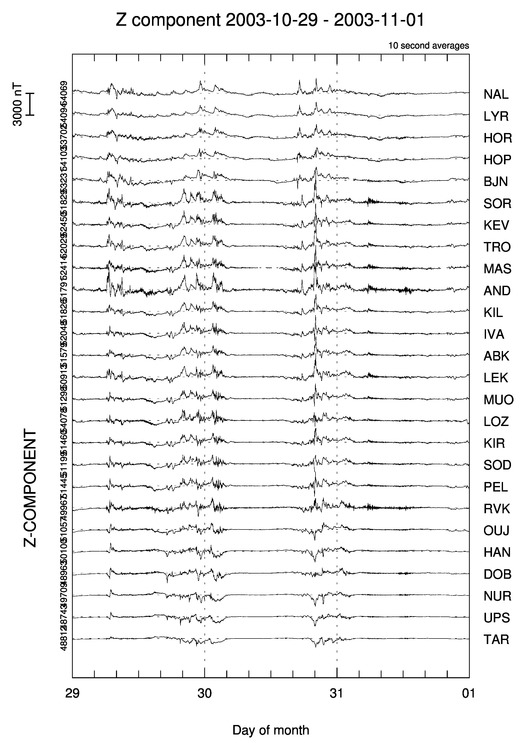
\includegraphics[width=\linewidth]{figures/IMAGE_Z_gram.jpg}
                \caption{\cite{image}.}
				\label{fig:image_z_gram}
        \end{subfigure}
        \caption{Pictures of animals}
        \label{fig:image_grams}
\end{figure}






sdfa









%----------------------------------------------------------------------------------------
%	EISCAT MADRIGAL (2).
%----------------------------------------------------------------------------------------
%\newpage
%----------------------------------------------------------------------------------------
%	EISCAT MADRIGAL.
%----------------------------------------------------------------------------------------

\section{EISCAT Madrigal}
example MISC \cite{exampleMISC}.\\
example Book \cite{exampleBOOK}.\\
example article \cite[p.~5]{exampleARTICLE}


%----------------------------------------------------------------------------------------
%	INTERNATIONAL REFERENCE IONOSPHERE (IRI) MODEL (1-2).
%----------------------------------------------------------------------------------------
\newpage 
\section{International Reference Ionosphere (IRI)}

This model has been developed by an international collaboration sponsored by the Committee on Space Research (COSPAR) and the international Union of Radio Science (URSE). The development started in the late sixties in order to create a standardized model of the ionosphere by compiling empirical data from the available sources at the time. this model has been updated several times  in order to keep it up to date with current measurements.
The data of IRI comes ionosondes, incoherent scatter radars, satellites and sounding rockets.
\newline
\newline
A comparison was made between the data from the IRI model and the data obtained with EISCAT's incoherent scatter radar in Svalbard, Norway. This comparison takes data at around 21:01 hours on the 30th of October of 2003, as part of the Halloween solar storms.

\begin{figure}[H]
	\centering
	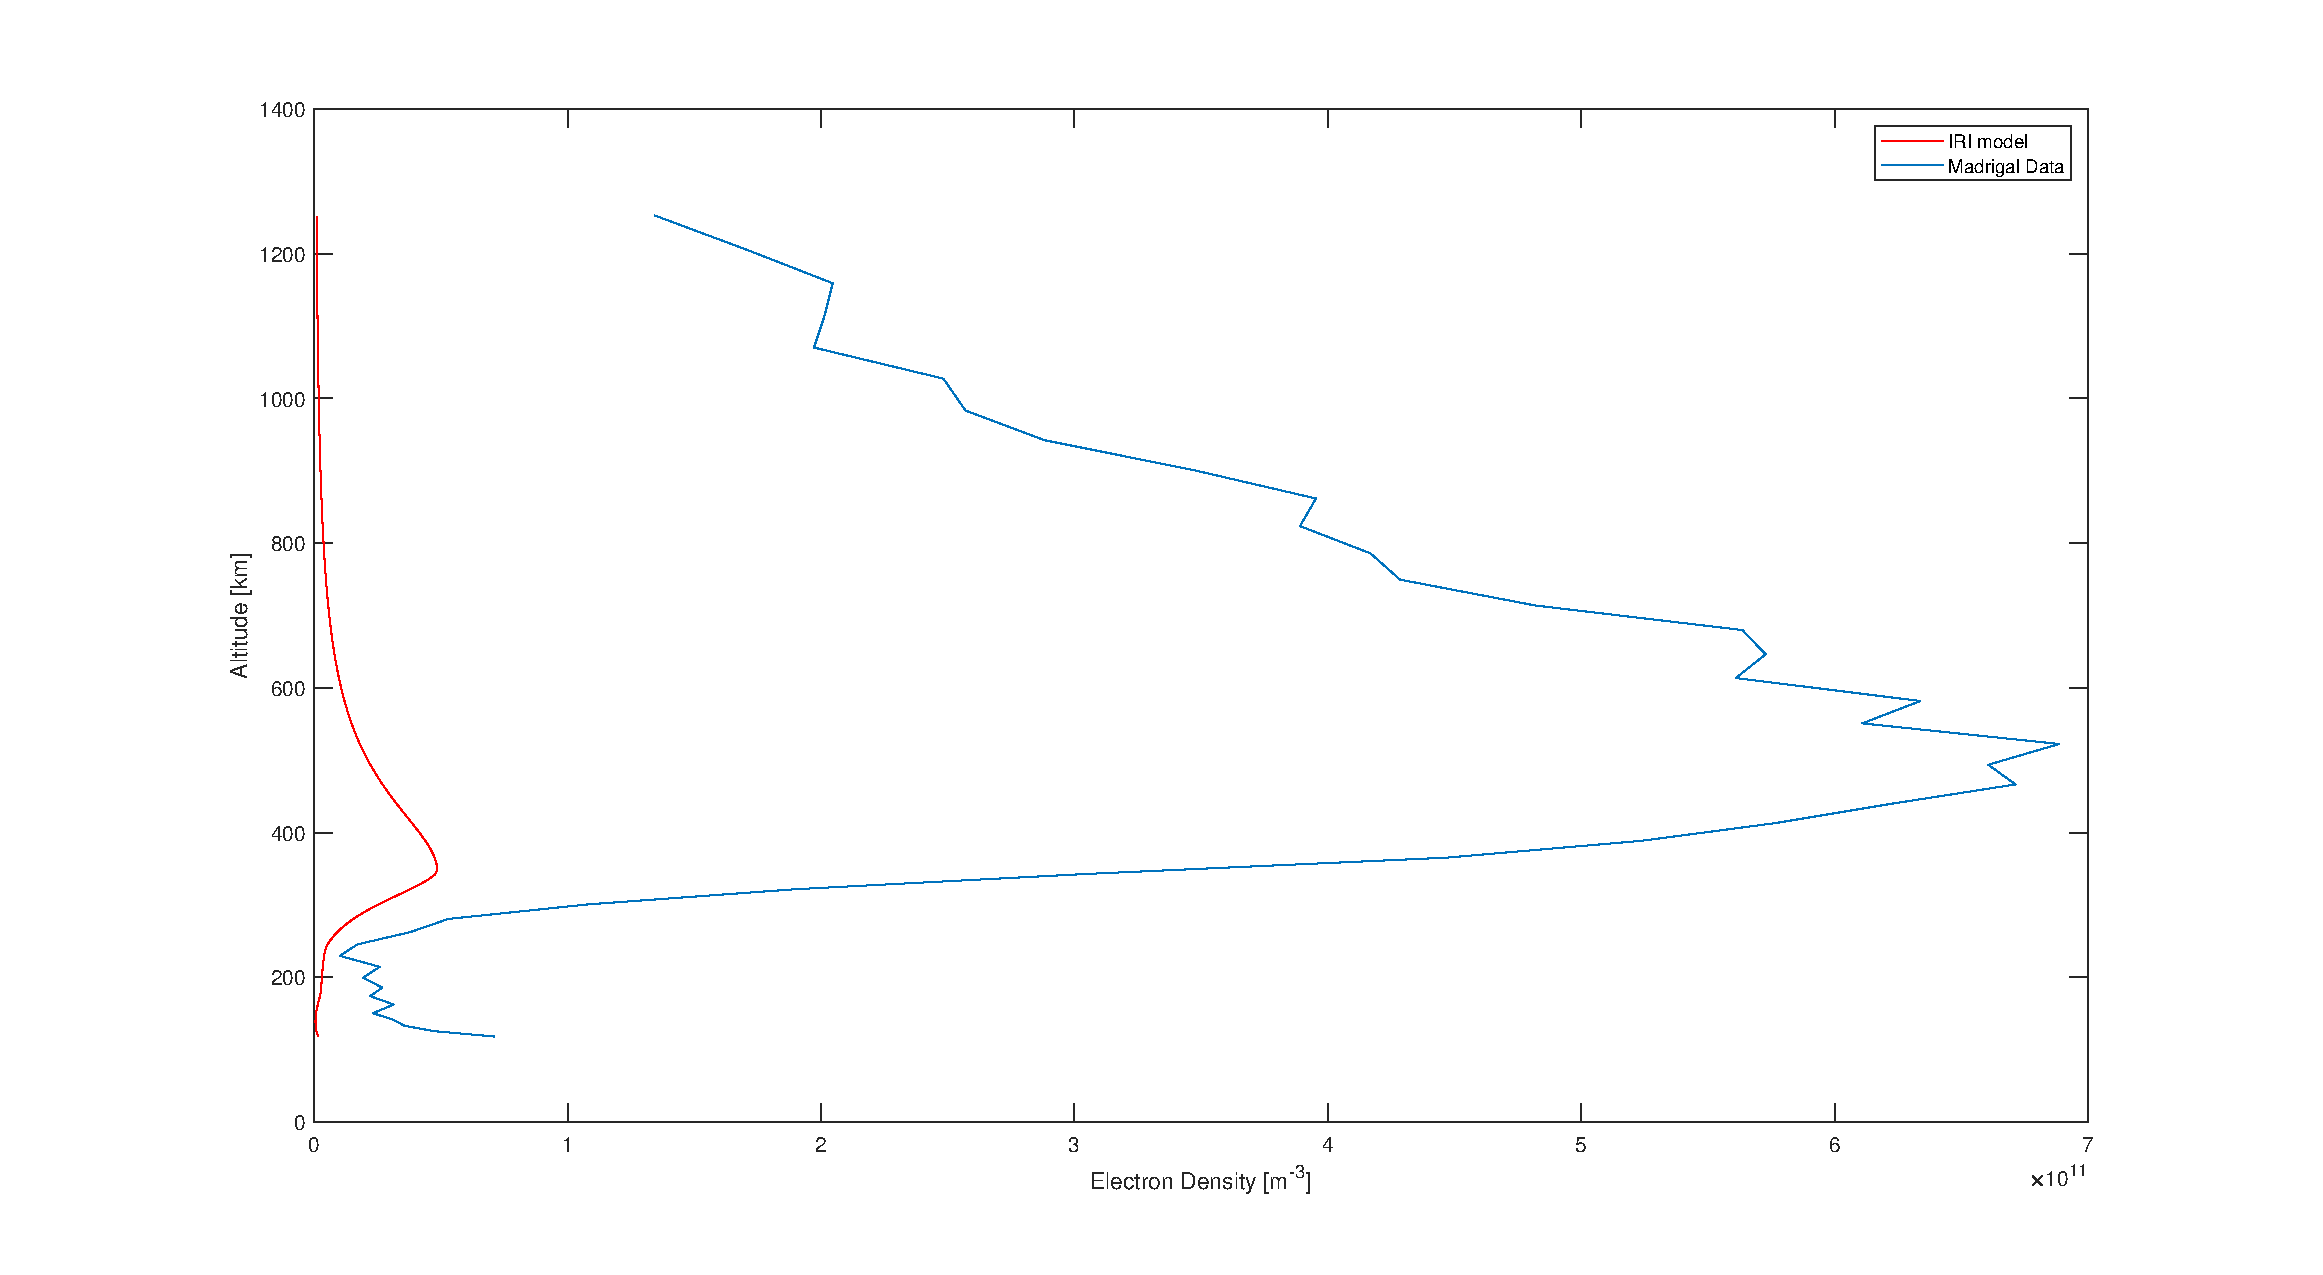
\includegraphics[height=14cm, width=\textwidth]{figures/IRIandMadrigalNe.eps}
	\caption{Comparison of the IRI model data (red) and the one obtained from EISCAT through the Madrigal system (blue).}
	\label{fig::IRIvsMa}
\end{figure}

While both sources more or less agree where the maximum of electron density occurs. There is a big discrepancy in the values shown, of about one order of magnitude.This can be attributed to the fact that the IRI model uses a monthly average to display the electron density of a particular time and date.


%----------------------------------------------------------------------------------------
%	DISCUSSION MADRIGAL AND IRI MODEL (1).
%----------------------------------------------------------------------------------------
\newpage
%----------------------------------------------------------------------------------------
%	DISCUSSION.
%----------------------------------------------------------------------------------------

\section{Discussion}
%example MISC \cite{exampleMISC}.\\
%example Book \cite{exampleBOOK}.\\
%example article \cite[p.~5]{exampleARTICLE}

The effects of solar flares are easily observed in Figure \ref{fig:madrigal}.
There is a strong increase in the electron density, a decrease in electron temperature, fluctuations in the ion temperatures, and changes in ion drift values.
Handzo \cite{Handzo} looked at X-class flares effects in the atmosphere and saw strongly increased electron density peaking after the the flare and the perturbation lasting a long time. This large difference between the actual electron density and the IRI-model estimate is shown in Figure \ref{fig::IRIvsMa}. The electron density during the storm is approximately a magnitude larger than the approximated model. The disturbance peaked after the solar flare and lasted for approximately an hour afterwards. After this time period, the electron density suddenly enters a depleted state with a lower electron density than prior to the flare.
The electron temperature is shown as decreased during and after the solar flare. This is contrary to the accepted notion of highest electron temperatures during the strongest solar storms \cite{Caspi}. This discrepancy between the the data shown and the expected results of the higher temperatures could be explained with differentiated plasma. This concept is explained in Battaglia \cite{Battaglia}, where there is cool core and the heated outer regions. Battaglia mentioned this could also be due to the cooler plasma in the foreground interacting with the higher temperature plasma.
During a solar flare, the ion temperatures can fluctuate during the solar storm due to positive and negative effects \cite{ITemp}. The ion temperature and the ion density interact interact causing an unpredictable variations. The temperature for the case of this Halloween storm fluctuated but remained higher than normal.
The solar flare has a positive and negative effect on $E \times B$ ion drift velocities \cite{IDrift}. There is a short lasting severe decrease in velocities and a longer lasting, much weaker increase in ion velocities.



%----------------------------------------------------------------------------------------
%	CONCLUSION (1).
%----------------------------------------------------------------------------------------
%----------------------------------------------------------------------------------------
%	CONCLUSION.
%----------------------------------------------------------------------------------------
\section{Conclusion}

In this report, the effects of the solar flares from Halloween 2003 on the ionosphere were analyzed and discussed. 
This report used data provided by EISCAT and Madrigad, to highlight and draw conclusions about the effects of solar flares on ionosphere.
The software used to analyze and create the graphs was GUISDAP by EISCAT in Matlab.
The effects of the flare were typical, and flare were clearly presented in the figures shown in the report. The electron density was almost a magnitude larger than the expected value from the IRI model.

%The effects of the storm were consequential but not severe in terms of health or technology impacts. This storm should serve as warning as the potential of a larger solar flare that could irreparably damage unprotected power grids or satellites. Damages to these systems could move human progress back decades.





%----------------------------------------------------------------------------------------
%	CONFIRMATION OF PARTICIPATION (1).
%----------------------------------------------------------------------------------------
\section{Confirmation of Participation}
Hereby, A. Hoehne, D. Talavera and E.F.M. Weterings declare to have participated and collaborated in this report.


%----------------------------------------------------------------------------------------
%	REFERENCES (1).
%----------------------------------------------------------------------------------------
\newpage				% Start at new page.
\addcontentsline{toc}{section}{References}
\printbibliography



\end{document}
